% This is samplepaper.tex, a sample chapter demonstrating the
% LLNCS macro package for Springer Computer Science proceedings;
% Version 2.20 of 2017/10/04
%
\documentclass[runningheads]{llncs}
%
\usepackage{graphicx}
\usepackage{multirow}
\usepackage{xcolor}
\usepackage{geometry}
\geometry{ margin=2cm, headsep=1cm, footskip=1cm }
% Used for displaying a sample figure. If possible, figure files should
% be included in EPS format.
%
% If you use the hyperref package, please uncomment the following line
% to display URLs in blue roman font according to Springer's eBook style:
% \renewcommand\UrlFont{\color{blue}\rmfamily}

\begin{document}
%
\title{Detecting Depression Levels using Deep Equilibrium Cascade with Feature Selection using Genetic Algorithm}
%
%\titlerunning{Abbreviated paper title}
% If the paper title is too long for the running head, you can set
% an abbreviated paper title here
%
\author{Chinh Duc La}
%
\authorrunning{Chinh Duc La}
% First names are abbreviated in the running head.
% If there are more than two authors, 'et al.' is used.
%
\institute{The Australian National University \\
Canberra, Australia\\
\email{u7098799@anu.edu.au}}
%\url{http://www.springer.com/gp/computer-science/lncs} \and
%ABC Institute, Rupert-Karls-University Heidelberg, Heidelberg, Germany\\
%\email{u7098799@anu.edu.au}}
%
\maketitle              % typeset the header of the contribution
%
\begin{abstract}
Depression is a serious mental illness problem. Detecting it too late could result in someone’s life. With the increasing trend in using neural networks for medical diagnosis, we try to use a neural network to detect depression levels using physiological signals from observers who watched some videos of depression patients. We use Genetic Algorithm to select features from dataset. Then, use Cascade Network\cite{casper_paper} with implicit layers inspired by Deep Equilibrium Networks \cite{deq_paper}. The performance of our model is surprisingly low with average accuracy of 31.7\% as we suspect this might be a problem from the dataset.

\keywords{Depression Detection  \and Neural Network \and Implicit Layer \and Cascade Network \and Genetic Algorithm \and Feature Selection.}
\end{abstract}
%
%
%
\section{Introduction}

Depression is one of many serious mental illnesses in the modern world that could result in someone’s death. However, depression is hard to detect as its symptoms are hard to notice, unlike many other conventional diseases. Detecting depression at early stages could save lives and maybe a better treatment result for depression patients. Normally, the diagnosis process requires a lot of questions from experts to detect depression levels. Sometimes, the diagnosis result also depends on how the patient’s answers. If we could have a different approach that requires less time and less expertise but reliable, we could have a better treatment for depression patients.

Neural network has been showing that it could perform at the superhuman level in some specific tasks. Many are trying to use neural networks for medical applications. For example, \cite{x_ray1_Bassi_2021} \cite{x_ray2_SAHA2021100505} try to diagnosis COVID-19 from chest X-ray images or \cite{Rajkomar2018}try to improve the healthcare system by predicting what to do next from Electronic Health Records or \cite{Esteva2017} could classify skin cancer at the dermatologist level using neural network. With the advancement in physiological technology, \cite{data_paper} could classify depression levels from physiological signals of observers with the accuracy of 88\% using only a simple neural network architecture and 92\% with the help of Genetic Algorithm to select features. In this paper, we will try to beat the previous result of \cite{data_paper}.

Feature selection could be seen as a combinatorial optimization problem with the objective of finding the best combination of input features that maximize some predefined goal. An exhaustive search for a subset of features that satisfy the problem could cost $O(2^{N})$ where $N$ is the number of input features. However, we could find a local optimal solution for this problem using Genetic Algorithm, an algorithm that was inspired by natural selection. Genetic Algorithm could find a really high quality solution through biological inspired operations like mutation, selection and crossover.

This paper do the following:
\begin{itemize}
    \item Using Genetic Algorithm to select features from dataset that work the best.
    \item Using data and training process from \cite{data_paper} to train and evaluate performance.
    \item Using the subset of features that is found by Genetic Algorithm to train Cascade neural network \cite{casper_paper} with modification from Deep Equilibrium Network \cite{deq_paper} with the hope for better performance.
\end{itemize}

\section{Methodology}
\subsection{Dataset}
We will use a subset of data from \cite{data_paper}, which consists of 192 data point (unlike the original data has 240 data point) that were extracted from physiological signals of 12 observers (original experiment has 14 observers) who watched videos of different depression level patients and rated depression level from 0 (no depression) to 3 (severe depression). Physiological signals were captured during the experiment are:
\begin{itemize}
    \item Galvanic Skin Response (GSR): convert into 23 features after feature extraction process.
    \item Pupillary Dilation (PD): convert into 39 features after feature extraction process.
    \item Skin Temperature (ST): convert into23 features after feature extraction process.
\end{itemize}
We have a total of 85 features extracted from all 3 signals. Upon inspecting dataset we have found something interesting. We use K-means Clustering to cluster the dataset and use 2 first principal components to visualize the dataset. From Figure \ref{fig:kmean} we can see that our clustering result and the label provided by the dataset don’t really match. Labels from the dataset likely to be random from the whole data space while the K-means clustering result is almost nicely clustered. The 2 clusters that are overlapping each other could be Mild and Moderate depression levels since \cite{data_paper} states that the performance of their model is not really good at these two categories or we can understand it as data points from these two categories are not nicely separated. As \cite{data_paper} states, ”our observers were not very good at consciously identifying the depression level of individuals in videos. . \textbf{The overall accuracy was 27\%} ...”. We think that the \textbf{label given in our dataset might be the label that was identified by observers, not the true labels}.
\begin{figure}
    \centering
    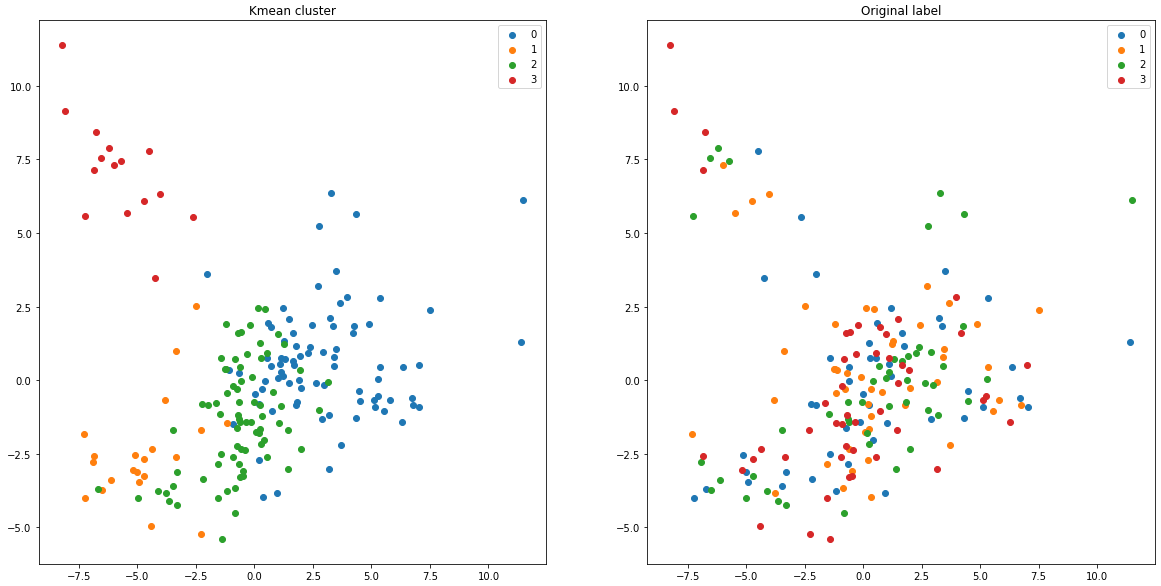
\includegraphics[width=0.8\textwidth]{kmean_vs_original.PNG}
    \caption{Left picture show clustering by K-means and original label (right picture) after being projected into 2 dimensions space by PCA}
    \label{fig:kmean}
\end{figure}

\subsection{Casper Algorithm}
Casper Algorithm \cite{casper_paper} is a constructive algorithm designed to overcome the limitation of Cascade Correlation algorithm (Cascor) \cite{cascor_paper}. Casper constructs the cascade networks the same way as Cascor: start with one hidden neuron and add a new hidden neuron after the loss function stops decreasing in the training process. But instead of freezing previous neurons that have been trained in trainning process like Cascor, Casper continues to train previously added neurons along with the newly added neuron but with adaptive learning rates based on the position of each neuron. The neural network will be divided into 3 regions:
\begin{itemize}
    \item \textbf{L1}: Connection from input, previously added neuron to the newly added neuron.
    \item \textbf{L2}: Connection from the newly added neuron to output of neural network
    \item \textbf{L3}: All the remaining connections.
\end{itemize}
\begin{figure}
    \centering
    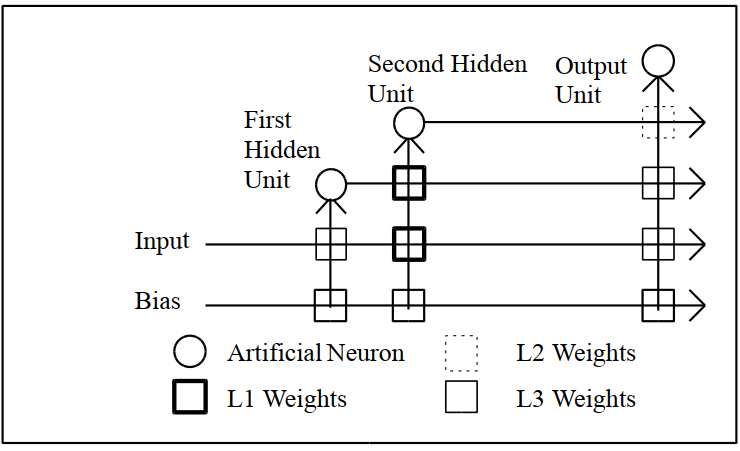
\includegraphics[scale=0.4]{casper_architecture.PNG}
    \caption{Casper architecture with 3 seperate regions (image from \cite{cascor_paper})}
    \label{fig:casper}
\end{figure}
The learning rate for each region is set to be $learning\_rate_1 >> learning\_rate_2 > learning\_rate_3$, where $learning\_rate_{i}$ is the learning rate for region $i$. The original paper uses resilient backpropagation (RPROP) but in this work, we will use RMSPROP \cite{rmsprop} to train our neural network.

\subsection{Implicit Layers}
Recent years have shown the success of implicit layers, a new class of layer of neural network where instead of computing the output explicitly as a function of input, implicit layer is defined as a problem satisfying some joint condition between input and output. Some of the problems could be differential equations \cite{neural_ode}, fixed point iteration \cite{deq_paper} or optimization solutions \cite{ddn}. Deep equilibrium models could be understand as we keep stacking layers until the output does not change no matter how many layers we keep adding. Due to cascade topology is somewhat similar to Deep equilibrium models (DEQ) \cite{deq_paper}. And \cite{bai2019trellis} had shown that network multiple layers that share the same weight could perform at the same level as different weight, we consider each hidden neuron of the cascade network is a fixed point iteration problem, which we could see as stacking many layers with same weights. In this work, We will use Anderson Acceleration\cite{anderson} to find fixed point of implicit layer (DEQ layer).
\begin{figure}
    \centering
    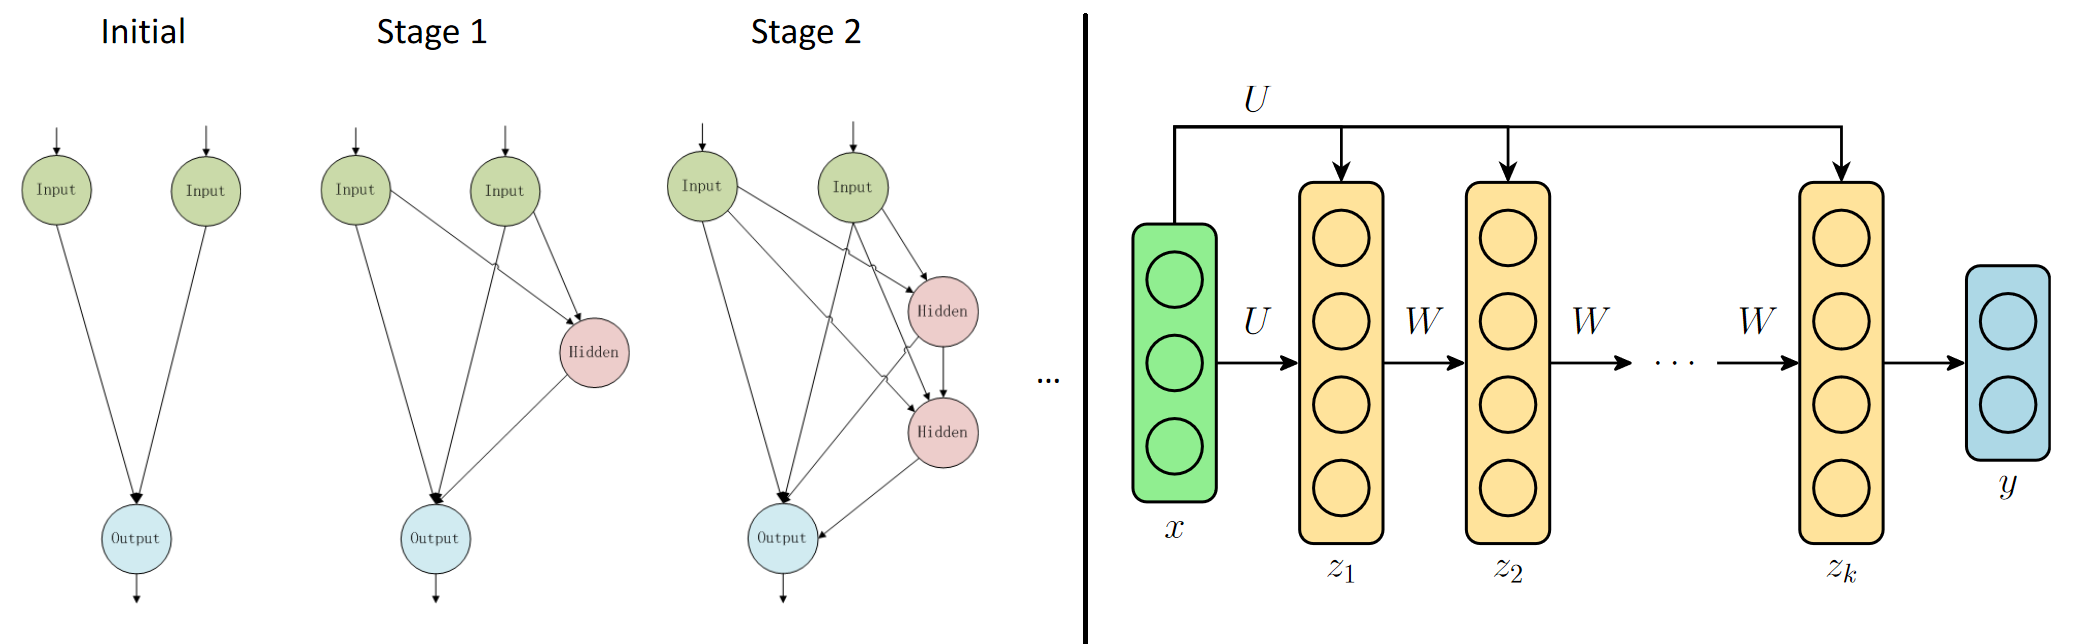
\includegraphics[width=0.8\textwidth]{cascade_topology.PNG}
    \caption{Cascade topology (left) with 2 neurons share the same topology with DEQ models (right) with 2 layers}
    \label{fig:my_label}
\end{figure}
\subsection{Genetic Algorithm for Feature Selection}
Genetic Algorithm (GA) is an algorithm that is inspired by natural selection. Genetic Algorithm is commonly used for optimization and search problems by relying on biologically inspired operators such as mutation, crossover and selection. In this work, we will use Genetic Algorithm to find a subset of features that could increase the model's performance. We will use $1$ in the chromosome as the feature is in the subset, and $0$ as it's not like showing in figure \ref{fig:ga_feature}. We use accuracy as a fitness function, and other settings for Genetic Algorithm is specified as Table \ref{tab:ga}.

\begin{figure}
    \centering
    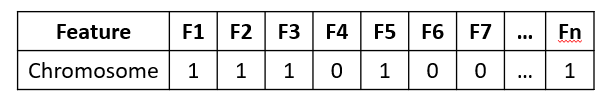
\includegraphics[scale=0.5]{GA_feature.PNG}
    \caption{An example of representation of chromosome for feature selection with Genetic Algorithm. Feature $F1, F2, F3, F5, Fn$ is in the selected subset, $F4, F6,F7$ is not in the chosen subset.}
    \label{fig:ga_feature}
\end{figure}
\begin{table}[h]
    \centering
    \caption{Genetic Algorithm Parameters}
    \begin{tabular}{|c|c|}
        \hline
        \textbf{Population} & 100 \\
        \hline
        \textbf{Generation} & 80\\
        \hline
        \textbf{Fitness} & Model's accuracy \\
        \hline
        \textbf{Crossover rate} & 0.8\\
        \hline
        \textbf{Mutation rate} & 1/85\\
        \hline
        \textbf{Crossover type} & Uniform crossover\\
        \hline
        \textbf{Mutation type} & Uniform mutation\\
        \hline
        \textbf{Selection type} & Stochastic universal sampling\\
        \hline
    \end{tabular}
    \label{tab:ga}
\end{table}

\subsection{Evaluation}
We will use Recall, Precision and F1 score as evaluation metrics for each depression level as our model evaluation. We use \textit{leave-one-patient-out} cross-validation for model selection. As when we train our model, we choose one patient's data for test, one patient's data for validation and the rest for training. Then, choose model with highest validation result to run on our test patient to get report result.
\section{Experiences}
\subsection{Implementation details}
We normalize data to have a mean of zero and a standard deviation of 1, to have a faster training process \cite{LeCun2012} \cite{NIPS2011_e836d813}. We use leave-one-patient-out cross validation to train neural networks and test their performance on Google Colab. We will implement 3 models:
\begin{itemize}
    \item \textbf{Baseline}: 1 hidden layer neuron network with 50 hidden neurons and sigmoid activation function and train with Adam optimization algorithm like in \cite{data_paper} and Dropout \cite{dropout}.
    \item \textbf{Casper}: a cascade neuron network with 40 hidden neurons and train with RMSProp
    \item \textbf{Fixed Point Casper}: A cascade neuron network with 2 hidden neurons. Each neuron is an implicit layer to solve fixed point problem and train with RMSProp
\end{itemize}
We use GA to find 12 different subsets for 12 folds of cross validation and combine 12 best bitstrings representing the presence of 85 features by counting how many times each feature appear in the best bitstrings then choose a threshold to choose whether or not to keep the feature (for example, if we choose threshold as $6$ which means we only choose features that appears at least 6 times from all 12 best subsets). Finally, we train 3 models again with the choosen subset and evaluate performance.

\subsection{Results}

\paragraph{\textbf{Training with full dataset}} Table \ref{tab1} show our experiment result. The final result is surprisingly lower than we expect. The baseline was implemented in \cite{data_paper} has an average accuracy of 88\% while our best baseline model only has the performance of 32.2\%. Recall, Precision, and F1 score are also low. F1 score is low because our model usually decided that it’s best to label all input with the same label, it makes Recall or Precision of that performance is zero which makes F1 score is also zero. 

Our Casper’s performance is even worse, with 23.9\% in average accuracy. However, Casper has shown that it could detect better with None and Severe depression levels and really bad at the other two. Fixed Point Casperperform quite well compared to baseline model in general although it but it is smaller in size.

When we tried to observe output from our models, we also realized that in many cases, both our Casper models also learned that it’s best to give a label for all input data. It makes us suspect the dataset might be the problem.
\begin{table}
\caption{Performance measure for depression recognition models defined from all Physiological signals}
\label{tab1}
\centerline{\begin{tabular}{|c|c|c|c|c|c|c|c|c|c|}
\hline
\multirow{2}{*}{\textbf{Depression level}} &  \multicolumn{3}{|c|}{\textbf{Baseline}} & \multicolumn{3}{|c|}{\textbf{Casper}} & \multicolumn{3}{|c|}{\textbf{Fixed Point Casper}}\\
\cline{2-10}
& Precision & Recall & F1 score & Precision & Recall & F1 score &  Precision & Recall & F1 score \\
\hline
None & 0.249 & 0.229 & 0.165 & 0.099 & \textbf{0.354} & 0.147 & \textbf{0.293} & \textbf{0.354} & \textbf{0.226}\\
\hline
Mild & \textbf{0.287} & 0.270 & 0.239 & 0.056 & 0.083 & 0.056 & 0.179 & \textbf{0.333} & 0.209\\
\hline
Moderate & 0.218 & \textbf{0.33} &  0.205 & 0.046 & 0.125 & 0.06 & \textbf{0.313} & 0.25 & 0.189\\
\hline
Severe & \textbf{0.424} & \textbf{0.458} & \textbf{0.332} & 0.102 & 0.395 & 0.162 & 0.24 & 0.313 & 0.228\\
\hline
Average & \textbf{0.294} & \textbf{0.322} & \textbf{0.235} & 0.076 & 0.239 & 0.106 & 0.256 & 0.313  & 0.213 \\
\hline
Overall Accuracy & \multicolumn{3}{|c|}{\textbf{0.322}} & \multicolumn{3}{|c|}{0.239} & \multicolumn{3}{|c|}{0.313}\\
\hline
\end{tabular}}
\end{table}

\paragraph{\textbf{Training with subset feature found by GA}} Table \ref{tab2} show the performance of our models when using a subset of feature generated by GA. Overall performance of all three models increases with Casper has a jump of 3.1\% in accuracy (from 23.9\% to 27\%). Baseline and Fixed Point Casper has a slight increase in average accuracy with 1.6\% and 0.4\% respectively. However, Baseline still have the highest performance comparing to the other two. This could mainly because we choose Baseline's performance as the fitness function for GA. Nonetheless, although we tried to find a subset that reflects the decision of the observers, our models' performance are still just better than randomly guessing by a small margin. Which means the distribution of each features with respect to each depression levels seems to be random. Therefore trying to find an optimal subset is not feasible.
\begin{table}
\caption{Performance measure for depression recognition models using a subset of features generated by GA}
\label{tab2}
\centerline{\begin{tabular}{|c|c|c|c|c|c|c|c|c|c|}
\hline
\multirow{2}{*}{\textbf{Depression level}} &  \multicolumn{3}{|c|}{\textbf{Baseline+GA}} & \multicolumn{3}{|c|}{\textbf{Casper+GA}} & \multicolumn{3}{|c|}{\textbf{Fixed Point Casper+GA}}\\
\cline{2-10}
& Precision & Recall & F1 score & Precision & Recall & F1 score &  Precision & Recall & F1 score \\
\hline
None & 0.284 & \textbf{0.562} & \textbf{0.333} & 0.041 & 0.166 & 0.066 & \textbf{0.322} & 0.437 & 0.292\\
\hline
Mild & 0.127 & 0.062 & 0.055 & 0.134 & 0.187 & 0.111 & \textbf{0.141} & \textbf{0.229} & \textbf{0.134}\\
\hline
Moderate & \textbf{0.370} & 0.291 & \textbf{0.279} & 0.104 & \textbf{0.416} & 0.166 & 0.188 & 0.208 & 0.137\\
\hline
Severe & \textbf{0.373} & \textbf{0.437} & \textbf{0.340} & 0.113 & 0.312 & 0.157 & 0.344 & 0.395 & 0.280\\
\hline
Average & \textbf{0.288} & \textbf{0.338} & \textbf{0.252} & 0.098 & 0.270 & 0.125 & 0.249 & 0.317 & 0.211\\
\hline
Overall Accuracy & \multicolumn{3}{|c|}{\textbf{0.338}} & \multicolumn{3}{|c|}{0.270} & \multicolumn{3}{|c|}{0.317}\\
\hline
\end{tabular}}
\end{table}

\section{Ablation Studies}

\paragraph{\textbf{Number of hidden neurons and model's performance}} Although \cite{deq_paper} stated that stacking DEQ layers does not increase the performance, the topology of Cascade network is still a little bit different. We tried to increase the total number of neurons of Fixed Point Casper to see if the performance of our model increase. The answer is no. As can be seen from figure \ref{fig:fpcp}, when the number of hidden neurons increases, the accuracy of the model fluctuates around 25\%-26\%.
\begin{figure}
    \centering
    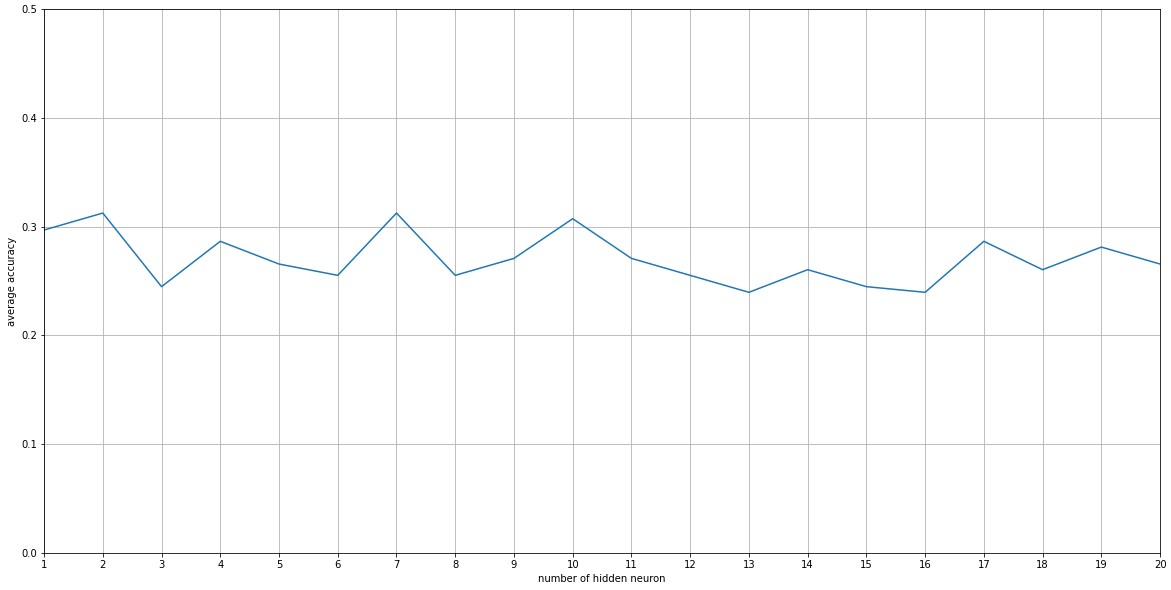
\includegraphics[width=\textwidth]{hidden_neuron.PNG}
    \caption{Number of neurons and average accuracy of Fixed Point Casper}
    \label{fig:fpcp}
\end{figure}

\paragraph{\textbf{Finding a subset of features that representing observers' prediction}} After inspecting the dataset, we have a hypothesis that the label in our dataset is not the true labels from the original dataset but the label the observers predicted. We want to find a subset of features that could reflect the prediction of observers better. However, the result is not as we predicted. The right figure of Figure \ref{fig:threshold} shows the number of features to keep with respect to each threshold. The left figure of Figure \ref{fig:threshold} shows something really interesting:
\begin{itemize}
    \item As the number of feature decreases, the average accuracy of Baseline increases, Fixed Point Casper decreases. The reason might be because we use accuracy of Baseline as the fitness function for  GA.
    \item Casper fluctuates around 25\% regardless the number of input features.
\end{itemize}
Modifying Casper to Fixed Point Casper changes the behavior of original Casper structure. More input features benefit Fixed Point Casper more than less input features. But, less irrelevant input features benefit Baseline. As a result, we could have a new development for this structure which is adding a hidden layer before start adding Fixed Point Cascade. The hidden layer could work as feature extraction from the subset to get more useful information so Fixed Point Cascade could work better.
\begin{figure}
    \centering
    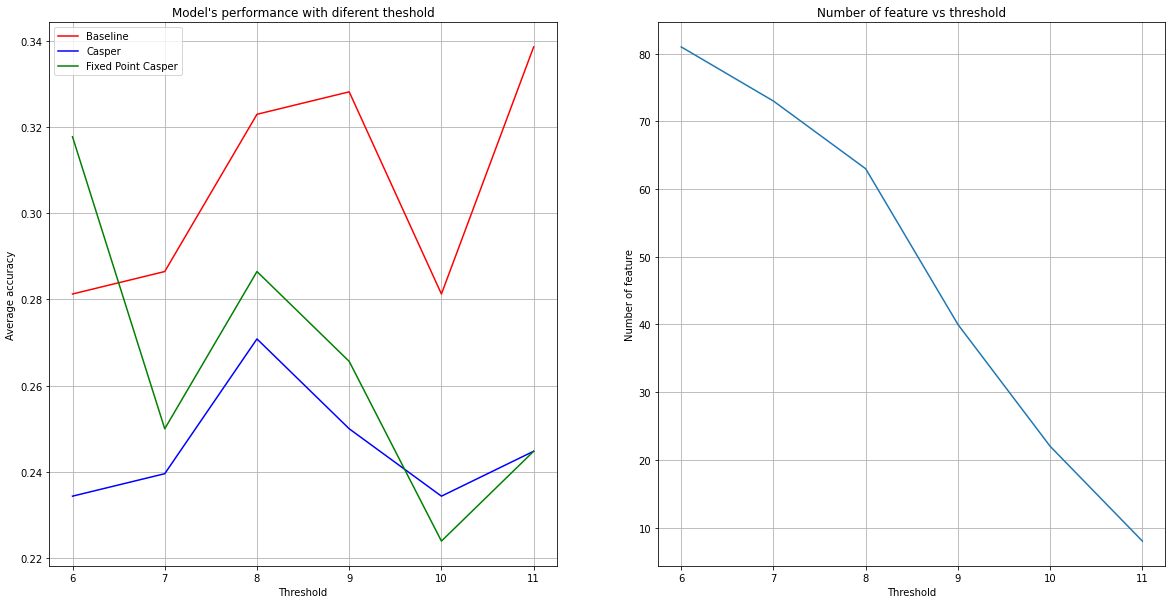
\includegraphics[width=\textwidth]{threshold.PNG}
    \caption{Caption}
    \label{fig:threshold}
\end{figure}

\section{Conclusion and Future Works}
We tried to Caper Algorithm and Fixed Point Casper to classify depression levels from physiology signals. Comparing to the Baseline model, Casper takes a longer time to train and Fixed Point Casper takes an even longer time with the same number of hidden neurons. Fixed Point Casper could perform with similar level to baseline model with smaller parameters (only 2 hidden neurons). However, we suspect that provided data might be incorrectly labeled so we cannot evaluate our model's performance. As a result, we tried to find a subset of features from the dataset that we believe that might reflect the way dataset was labeled using Genetic Algorithm. The Performance did increase but not as much as we expect. But, Fixed Point Casper works better when there are more input features while Baseline work better when choosing only relevant subset. So we could add a hidden layer before adding Fixed Point Cascade Neuron to make use of the infromation extraction from a single hidden layer. Another problem we want to address is the label of the provided dataset which we believe is incorrect, we could do some data preprocessing using information from \cite{data_paper} such as the highest the accuracy of prediction from observer with respect to each label and Kmeans to try to recover the true label.
%
% ---- Bibliography ----
%
% BibTeX users should specify bibliography style 'splncs04'.
% References will then be sorted and formatted in the correct style.
%
% \bibliographystyle{splncs04}
% \bibliography{mybibliography}
%
\bibliographystyle{splncs04}
\bibliography{references}
\end{document}
